\documentclass{article}
\usepackage[polish]{babel}
\usepackage[utf8]{inputenc}
\usepackage{polski}
\frenchspacing
\setcounter{tocdepth}{2}
\usepackage{graphicx}
\graphicspath{ {images/} }
\usepackage{float}
\usepackage{listings}
\usepackage{hyperref}

\usepackage{booktabs}% http://ctan.org/pkg/booktabs
\newcommand{\tabitem}{~~\llap{\textbullet}~~}

\linespread{1.3}
\frenchspacing

\setcounter{tocdepth}{3}

\begin{document}

% -------------------------- TITLEPAGE -------------------------- %

\begin{titlepage}

\newcommand{\HRule}{\rule{\linewidth}{0.5mm}}

\begin{center}

% university
\textsc{\LARGE Politechnika Warszawska}\\[0.5cm]
\textsc{\Large Wydział Matematyki i Nauk Informacyjnych}\\[1cm]

% logo

\includegraphics[width=2cm, height=2cm]{logo}\\[1cm]


\textsc{\Huge Wstęp do algorytmów ewolucyjnych}\\[0.5cm]

%----------------------------------------------------------------------------------------

\HRule \\[0.4cm]
{ \LARGE \bfseries Wielostartowy algorytm wspinaczkowy dla ciągłych zadań optymalizacji o różnych wymiarowościach}\\[0.2cm]
 
%----------------------------------------------------------------------------------------

\HRule \\[0.4cm]
{  \bfseries RAPORT}\\[2.5cm]

% author
\begin{flushright}
	\Large \emph{Autorzy:}\\[0.5cm]
Anna \textsc{Zawadzka}\\
Piotr \textsc{Waszkiewicz}\\[1.5cm]
\end{flushright} 

% date
\vfill
{\large \today}\\[1cm]
	
\end{center}

\end{titlepage}

\newpage
%----------------------------------------------------------------------------------------
\section{Opis problemu}

Celem projektu było zbadanie zachowania wielostartowego algorytmu wspinaczkowego dla ciągłych zadań optymalizacji o różnych wymiarowościach z uwzględnieniem rożnych strategii losowania punktów startowych: losowanie z rozkładem równomiernym, przeszukiwanie po hipersiatce, poisson-disc. Testy przeprowadzone zostały na benchmarku CEC 2013.\\

Podczas działania algorytmu wspinaczkowego można napotkać takie problemy jak: lokalne minima, \textit{plateaux}, czyli równiny oraz wąskie grzbiety. W niektórych problemach mogą pomóc wielokrotne starty z różnych punktów, stąd cel tego zadania - sprawdzenie które podejście może zminimalizować ryzyko nieodnalezienia poszukiwanego globalnego ekstremum.

\section{Metoda realizacji zadania}

\subsection{Algorytm wspinaczkowy}

W projekcie wykorzystany został algorytm wspinaczkowy w wersji z wyborem następnika na podstawie sąsiadów najlepszego znalezionego dotychczas punktu. \\
Należy zaznaczyć, że wszystkie funkcje w pakiecie CEC 2013 realizują problem minimaizacji.

\begin{lstlisting}[mathescape][language=R]
x $\leftarrow$ $x_{0}$
while !stop
	y $\leftarrow$ randomNeighbor(x, $\delta$)
	if cec2013(i, y) < cec2013(i, x)
		x $\leftarrow$ y
\end{lstlisting}
Dodatkowo zaimplementowany algorytm zapisuje wartość funkcji celu dla każdego osobnika. Warunkiem stopu jest osiągnięcie ektremum globalnego, bądź zatrzymanie się w lokalnym ekstremum na czas 100 iteracji.\\

Funkcja \textit{randomNeighbor(x, $\delta$)} zwraca losowy punkt w sąsiedztwie $x$-a, znajdujący się w odległości nie większej niż $\delta$ od $x$-a. Do obliczania odległości stosowana jest metryka euklidesowa. W przypadku wygenerowania punktu, który znajdue się poza dopuszczalnym obszarem, jest on korygowany przy pomocy metody zawijania.\\

Funkcja \textit{cec2013(i, z)} dostępna jest w ramach pakietu CEC2013 i zwraca wartość funkcji $i$ w punkcie $z$. Traktowana jest jako funkcja celu.


\subsection{Strategie losowania punktów startowych}
Punkty startowe wybierane są przy pomocy następujących metod:

\subsubsection{Losowanie z rozkładem równomiernym}
Rozkład równomierny gwarantuje wybranie punktu z określonej n-wymiarowej przestrzeni z jednakowym prawdopodobieństwem. Środowisko R dostarcza funkcję \textit{runif(n, a, b)}, która zwraca n liczb z przedziału [a,b] z rozkładu równomiernego, które traktowane są jako kolejne współrzędne generowanego punktu.

\subsubsection{Przeszukiwanie po hipersiatce}
Metoda ta zakłada istnienie n-wymiarowej siatki. Przecięcia linii tejże siatki wyznaczają kolejne punkty, będące punktami startowymi algorytmu.

\subsubsection{Poisson Disc Sampling}
Technika Poisson Disc generuje zbiór punktów o zadanej liczności w n-wymiarowej przestrzeni, ściśle upakowanych, lecz odległych od siebie co najmniej o podaną minimalną odległość. Algorytm zrealizowany został zgodnie z metodą podaną w poniższym dokumencie:\\
\url{http://www.cs.ubc.ca/~rbridson/docs/bridson-siggraph07-poissondisk.pdf}

\newpage
\section{Przebieg eksperymentów}

Funkcja cec2013 dostarczona w ramach pakietu CEC2013 przyjmuje dwa argumenty: punkt oraz numer funkcji wykorzystanej do obliczenia wartości funkcji celu dla podanego punktu. Dostępne funkcje numerowane są od 1 do 28, a podany punkt musi być punktem z przestrzeni o wymiarze 2, 5, 10, 20, 30, 40, 50, 60, 70, 80, 90 lub 100. Daje to 336 doświadczeń, które dodatkowo przeprowadzane są dla każdej z trzech strategii losowania punktów startowych, co daje 1008 eksperymentów. Liczba doświadczeń przez nas przeprowadzonych jest jednak mniejsza ze względu na dużą złożoność czasową obliczeń. Ponadto generowanie punktów metodą Poisson Disc zrealizowane jest tylko dla przestrzeni 2 i 5-wymiarowej ze względu na bardzo dużą złożoność pamięciową.\\
Do eksperymentów zostały wybrane wymiary: 2, 5, 10 oraz funkcje: 1, 8, 12, 6. Poniższa tabela przedstawia wartości ekstremów globalnych wybranych funkcji (realizujemy problem minimaizacji).\\
\begin{center}
\begin{tabular}{|r|r|}
  \hline 
  numer funkcji & minimum funkcji celu\\
  \hline 
  1 & -1400\\
  \hline
  8 & -700 \\
  \hline
  12 & -300 \\
  \hline
  6 & -900 \\
  \hline
\end{tabular}
\end{center}
Funkcje te zostały wybrane na podstawie analizy poniższego dokumentu, który zawiera opisy i wizualizacje wszystkich dostępnych w pakiecie funkcji:\\
\url{http://www.ntu.edu.sg/home/EPNSugan/index_files/CEC2013/Definitions%20of%20%20CEC%2013%20benchmark%20suite%200117.pdf} \\
Pierwsze dwie wybrane funkcje (1 i 8) mają dobrze widoczne ekstremum globalne, funkcja 12 jest funkcją nietrywialną z wielona ekstremami lokalnymi, natomiast funkcja 6 jest płaska na znaczącej części przestrzeni.
\newpage
Poniższe szkice przedstawiają wykresy wybranych funkcji:\\

\begin{figure}[H]
\centering
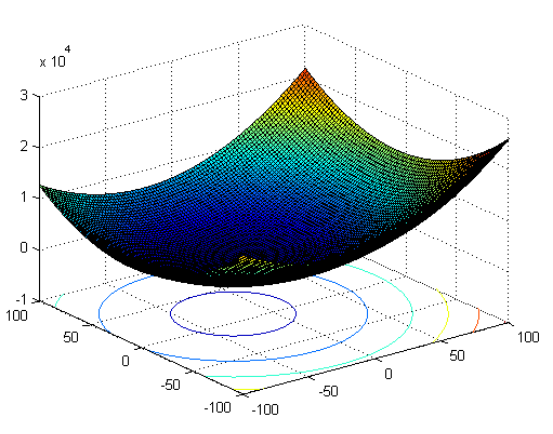
\includegraphics[scale=0.6]{1}
\caption{Wykres funkcji nr 1}
\end{figure}

\begin{figure}[H]
\centering
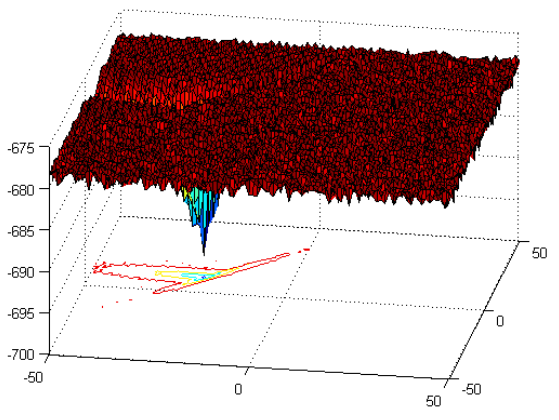
\includegraphics[scale=0.6]{8}
\caption{Wykres funkcji nr 8}
\end{figure}


\begin{figure}[H]
\centering
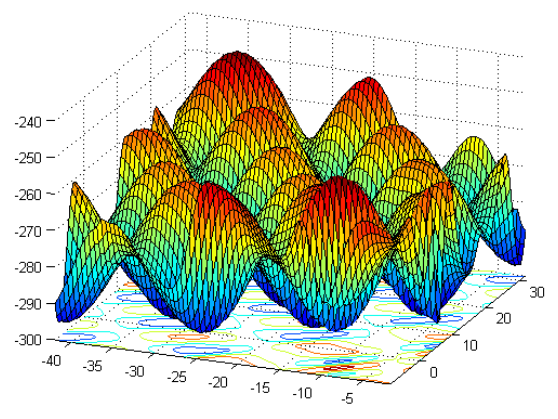
\includegraphics[scale=0.6]{12}
\caption{Wykres funkcji nr 12}
\end{figure}


\begin{figure}[H]
\centering
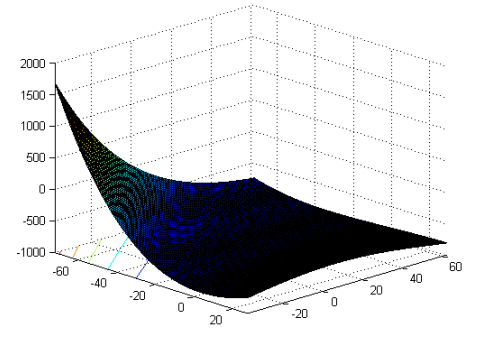
\includegraphics[scale=0.7]{6}
\caption{Wykres funkcji nr 6}
\end{figure}
\newpage
Ogólna postać głównego algorytmu:\\
\begin{lstlisting}[mathescape][language=R]
dimensions $\leftarrow$ c(2,5,10);
functions $\leftarrow$ c(1,8,12,6);
foreach d in dimensions
    NumberOfPoints $\leftarrow$ 10*d;
    S1 $\leftarrow$ starting points set - uniform distribution;
    S2 $\leftarrow$ starting points set - hyper mesh;
    S3 $\leftarrow$ starting points set - poisson disc;
    foreach f in functions)
        run hillClimbing for d, f, S1;
        run hillClimbing for d, f, S2;
        run hillClimbing for d, f, S3;
\end{lstlisting}

Algorytm wspinaczkowy wywyoływany jest dla każdego punktu ze zbioru punktów startowych, po czym następuje wyliczenie wartości średnich na podstawie wyników otrzymanych dla każdego z punktów startowych.\\
Ponieważ testowana metoda jest niedeterministyczna, każde doświadczenie jest powtarzane 20 razy, a wyniki uśredniane.\\


\section{Wyniki eksperymentów}
Poniższe wykresy przedstawiają wartości funkcji celu dla kolejnych najlepszych osobników w populacji. Kolorem czerwonym zaznaczono wyniki dla metody z losowaniem punktów startowych z rozkładem równomiernym, kolorem zielonym - metodę z przeszukiwaniem po hipersiatce, a kolorem niebieskim - metodę bazującą na Poisson Disc. Dla każdej z funkcji przedstawione zostały 3 wykresy (dla każdego z trzech rozpatrywanych wymiarowości przestrzeni), przy czym na wykresach dla wymiaru 10 zwizualizowano wyniki dla dwóch metod losowania punktów startowych (metoda z losowaniem punktów startowych z rozkładem równomiernym oraz metoda z przeszukiwaniem po hipersiatce).

\subsection{Funkcja nr 1}


\begin{figure}[H]
\centering
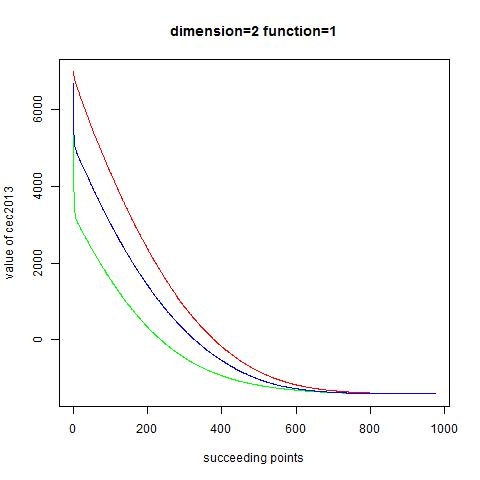
\includegraphics[scale=0.6]{dim_2__func_1}
\caption{Wyniki dla funkcji 1 i wymiaru 2}
\end{figure}

\begin{figure}[H]
\centering
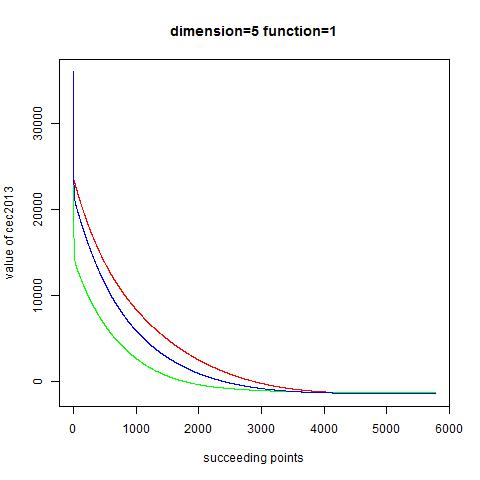
\includegraphics[scale=0.6]{dim_5__func_1}
\caption{Wyniki dla funkcji 1 i wymiaru 5}
\end{figure}

\begin{figure}[H]
\centering
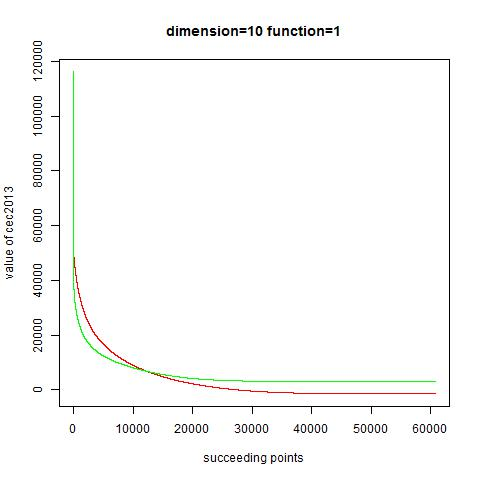
\includegraphics[scale=0.6]{dim_10__func_1}
\caption{Wyniki dla funkcji 1 i wymiaru 10}
\end{figure}

\subsection{Funkcja nr 8}


\begin{figure}[H]
\centering
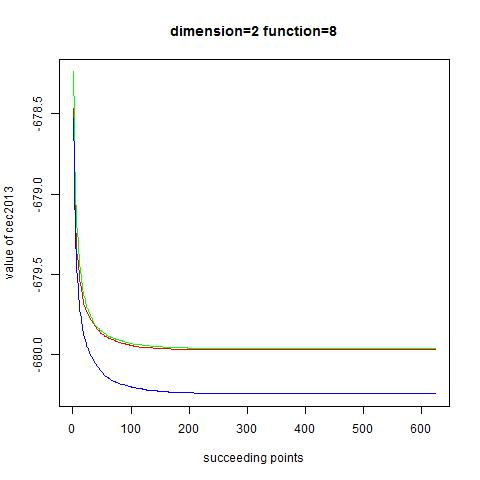
\includegraphics[scale=0.6]{dim_2__func_8}
\caption{Wyniki dla funkcji 8 i wymiaru 2}
\end{figure}

\begin{figure}[H]
\centering
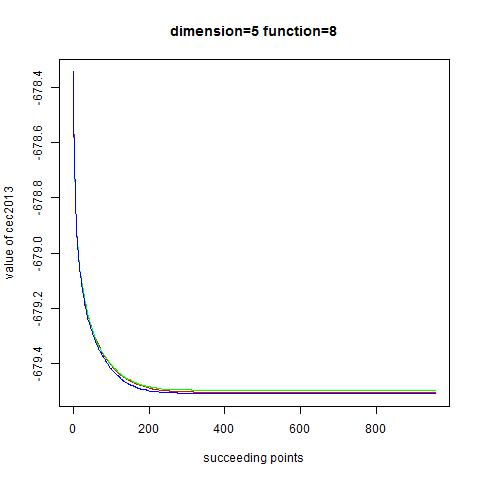
\includegraphics[scale=0.6]{dim_5__func_8}
\caption{Wyniki dla funkcji 8 i wymiaru 5}
\end{figure}

\begin{figure}[H]
\centering
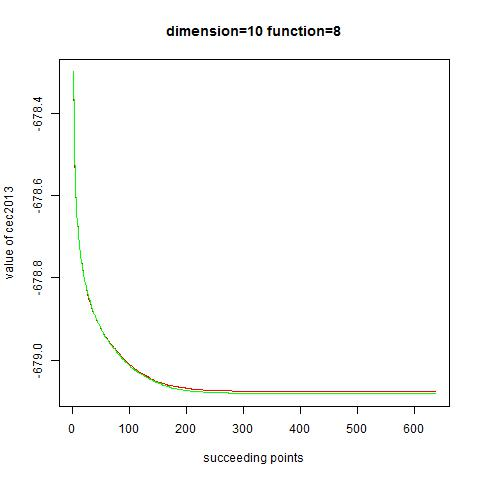
\includegraphics[scale=0.6]{dim_10__func_8}
\caption{Wyniki dla funkcji 8 i wymiaru 10}
\end{figure}

\subsection{Funkcja nr 12}


\begin{figure}[H]
\centering
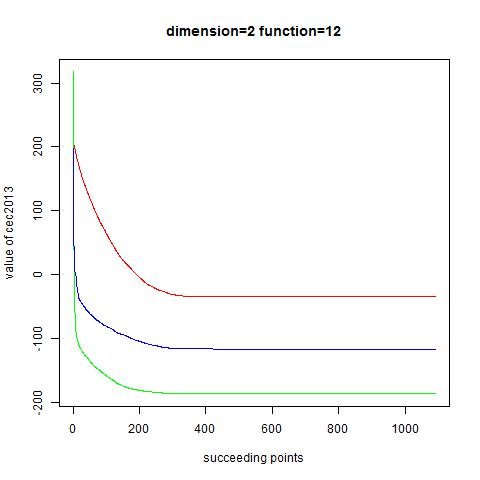
\includegraphics[scale=0.6]{dim_2__func_12}
\caption{Wyniki dla funkcji 12 i wymiaru 2}
\end{figure}

\begin{figure}[H]
\centering
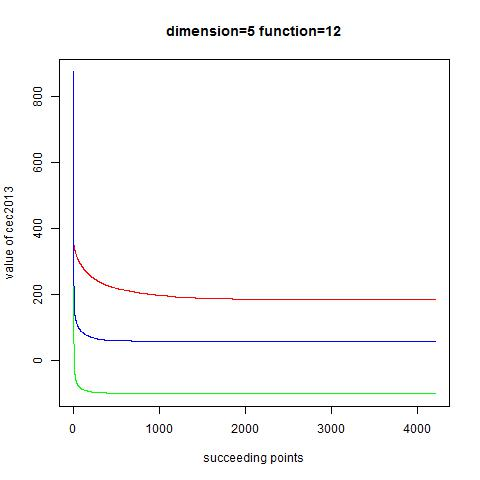
\includegraphics[scale=0.6]{dim_5__func_12}
\caption{Wyniki dla funkcji 12 i wymiaru 5}
\end{figure}

\begin{figure}[H]
\centering
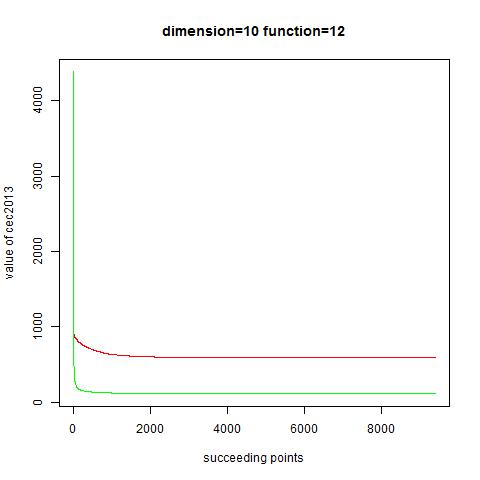
\includegraphics[scale=0.6]{dim_10__func_12}
\caption{Wyniki dla funkcji 12 i wymiaru 10}
\end{figure}

\subsection{Funkcja nr 6}


\begin{figure}[H]
\centering
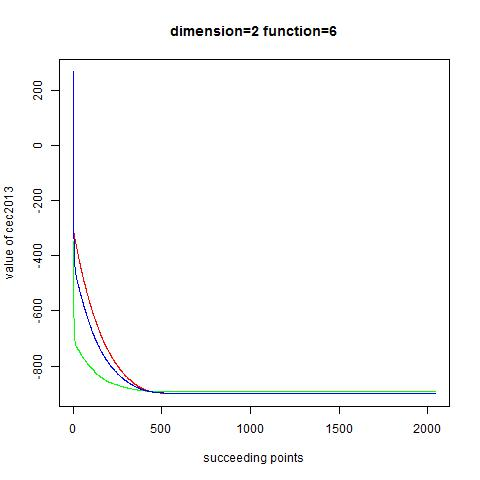
\includegraphics[scale=0.6]{dim_2__func_6}
\caption{Wyniki dla funkcji 6 i wymiaru 2}
\end{figure}

\begin{figure}[H]
\centering
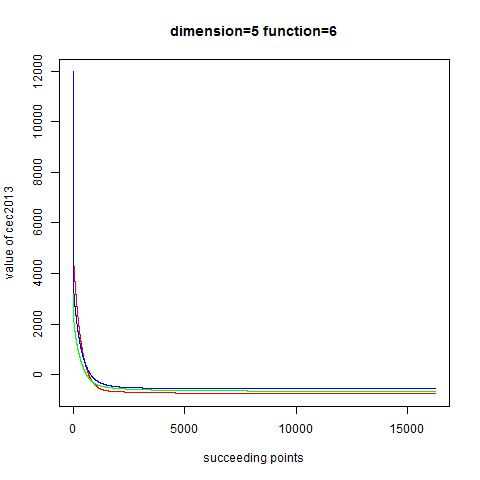
\includegraphics[scale=0.6]{dim_5__func_6}
\caption{Wyniki dla funkcji 6 i wymiaru 5}
\end{figure}

\begin{figure}[H]
\centering
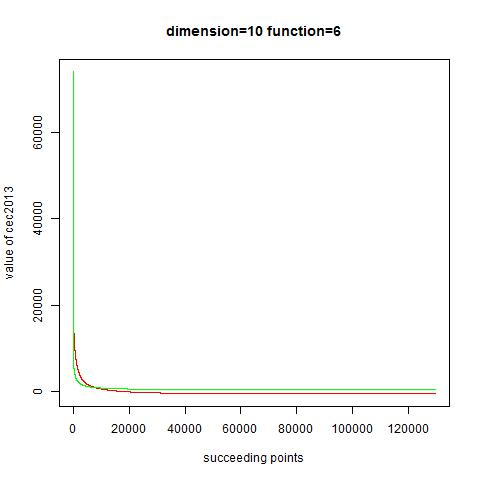
\includegraphics[scale=0.6]{dim_10__func_6}
\caption{Wyniki dla funkcji 6 i wymiaru 10}
\end{figure}

\section{Wnioski}

Na podstawie przeprowadzonych eksperymentów z pewnością możemy stwierdzić, że wielokrotne uruchomienie algorytmu wspinaczkowego z różnych punktów startowych przyczynia się do uzyskania lepszych wyników, niż rozpatrzenie jednego punktu startowego. Takie podejście zwiększa szanse na to, że globalne ekstremum zostanie osiągnięte i zmniejsza ryzyko zatrzymania się w ekstremum lokalnym.\\
Wyniki przeprowadzonych doświadczeń pokazują, że metoda wyboru punktów startowych powinna być uzależniona od funkcji celu, nie można jednoznacznie stwierdzić, że pewna konkretna metoda będzie dawała najlepsze wyniki dla wszystkich funkcji.


\end{document}